\pagebreak
\subsection{Universal Synchronous Asynchronous Receiver Transmitter (USART)}
La prima periferica usata è stata la USART. Usart ci permette di comunicare con il PC attraverso la Seriale.
\\

\subsubsection{Funzionamento}
Seppur la periferica permetta il trasferimento sicrono dei dati, noi la useremo come USART, quindi una versione precedente.\\

Questa periferica per funzionare ha bisogno di un collegamento diretto con il dispositivo a cui comunicare, questo collegamento nel nostro cavo consiste in 3 cavi: TX, RX e GND.\\

\noindent
\begin{minipage}[c]{0.54\linewidth}
    \begin{itemize}
        \item TX: Trasmettitore, invia i dati al PC
        \item RX: Ricevitore, riceve i dati dal PC
        \item GND: Collegamento a terra, serve per chiudere il circuito e tarare entrambi i dispositivi allo stesso 0
    \end{itemize}
\end{minipage}
\hfill
\begin{minipage}[t]{0.4\linewidth}

    \centering
    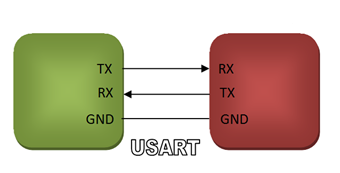
\includegraphics[width=0.7\linewidth]{microcontrollore/assets/USART.png}
    \label{fig:USART}
    \captionof{figure}{Collegamento tra microcontrollore e PC}
\end{minipage}

I dati sono mandati sottoforma di impulsi elettrici. Dato che i due dispositivi sono collegati con un singolo cavo, i dati sono inviati in ordine e, l'unica cosa di cui i due dispositivi hanno bisogno è la velocità di trasmissione, che deve essere uguale tra i 2 per assicurare la giusta lettura.\\
La velocità di trasmissione è misurata in baud, ovvero il numero di bit trasmessi in un secondo e per questo si chiama Baud Rate. Di base è a 9600 baud, ma a seconda delle necessità può essere alzata fino al limite strumentale.\\

Per evitare problemi di lettura, il ricevitore overcampiona i dati per poi farne una media. Così facendo, il rumore dovuto a cavi troppo lunghi o a interferenze elettromagnetiche viene minimizzato.\\


\subsubsection{Programmazione}
Usart, nel nostro caso, è stato usare nel seguente modo: Inizialmente abbiamo spedito un carattere specifico dal pc al microcontrollore, questo carattere l'abbiamo usato come trigger per far partire la lettura dei dati, finita la lettura dei dati abbiamo trasmesso tutti i dati al computer.\\

\noindent
\begin{minted}[bgcolor = coding, linenos]{C}
void ESPE_USART_char_start(void){

    if ( USART3 ->ISR & USART_ISR_RXNE_RXFNE){ // Se il buffer è pieno
        if ( USART3 -> RDR == char_trigger){ // Se il carattere è uguale al trigger
            flag_Trigger_EN = 1;

        }
    }
}
\end{minted}
\label{code:USART_start}

Nel codice \ref{code:USART_start}, andiamo ad usare 2 registri di USART: ISR e RDR. Il primo, l'Interrupt Status Register, contiene flag per controllare lo status di USART, mentre il secondo, il Receive Data Register, contiene il dato ricevuto.\\

\noindent
\begin{minted}[bgcolor = coding, linenos]{C}
#define len_vec 100
uint_8 vec_dati[len_vec];
uint_8 len = sizeof(uint_8)/sizeof(char)*len_vec;
char *str = vec_dati;
uint_8 indice = 0;


void ESPE_USART_send_data(void){
    if( USART3 ->ISR & USART_ISR_TC){ // Se il buffer è vuoto
		if (indice < len){
			USART3->TDR = *(str+indice); // Invia il dato
			indice++;
		}else{
			if(indice == len){
				USART3 -> TDR = '\r'; // Invia il carattere di fine riga
				indice = 0;
			}
		}
	}
}
\end{minted}
\label{code:USART_send}

In questo codice, invece andiamo a usare il registro TDR, il Transmission Data Register, per mandare i dati al PC, ma, dato che i dati sono messi in un vettore di uint8 e il TDR ha le dimensioni di un char, il numero di byte da inviare non corrisponde alla dimensione del vettore. Questa discrepanza è risolta dalla variabile *str che è una variabile puntatore di tipo char puntata all'inizio del vettore.\\


Oltre a queste funzioni è necessario definire un'altra funzione ausiliaria con la quale si passa dalla lettura dei dati al loro invio.\\

\noindent
\begin{minted}[bgcolor = coding, linenos]{C}
void ESPE_USART_invert_mode(void){
    if(USART3 -> CR1 & USART_CR1_RXNEIE){
        USART3 -> CR1 &= ~USART_CR1_RXNEIE;
        USART3 -> CR1 |= USART_CR1_TCIE;
    }else if(USART3 -> CR1 & USART_CR1_TCIE){
        USART3 -> CR1 |= USART_CR1_RXNEIE;
        USART3 -> CR1 &= ~USART_CR1_TCIE;
    }
}
\end{minted}

Questa funzione cambia il metodo di trigger dell'interrupt di USART, così facendo si evitano problemi di trigger dell'interrupt in lettura mentre l'invio è in corso o viceversa.\\


